\documentclass[12pt,fleqn]{article}
\setlength{\parindent}{0pt}
\usepackage{graphicx}
\usepackage{listings}
\usepackage[latin5]{inputenc}
\setlength{\parskip}{8pt}
\setlength{\parsep}{0pt}
\setlength{\headsep}{0pt}
\setlength{\topskip}{0pt}
\setlength{\topmargin}{0pt}
\setlength{\topsep}{0pt}
\setlength{\partopsep}{0pt}
\setlength{\mathindent}{0cm}

\begin{document}
MIT OCW Cok Degiskenli Calculus - Ders 9

Bu dersin konusu birden fazla degisken iceren fonksiyonlarin minimizasyonu
ile ugrasirken yardimci olacak kismi turev (partial derivative)
kavrami. Cok degiskenli bir fonksiyon $f(x,y)$'nin birden fazla turevi
vardir. Mesela bunlardan bir tanesi

\[ \frac{\partial f}{\partial x} = f_x \]

Bu turev $x$'in degistirildigi ama $y$'nin sabit tutuldugu bir durumu
gosterir. 

\[ \frac{\partial f}{\partial y} = f_y \]

ise $y$'in degistirildigi ama $x$'nin sabit tutuldugu bir durumu gosterir.

Simdi her ikisinin birden degistirildigi durumda ne olacagini gosteren
yaklasiksal (approximate) formulu gorelim. Degisim matematiksel olarak
soyle

\[ x \sim x + \Delta x \]

\[ y \sim x + \Delta x \]

O zaman $z$ icin

\[ z = f(x,y) \]

yaklasiksal degisim soyle olur

\[ \Delta z \approx f_x\Delta x + f_y \Delta f_y \]

Tekrar vurgulamak gerekirse bu yaklasiksal bir formul, daha ``dogru'' bir
temsil icin 2., 3. turevleri iceren daha yuksek dereden (higher order
terms) terimlerin de olmasi gerekir, fakat bu terimler 1. derece lineer bir
yaklasiksallik icin kullanilmaz. 

Bu formulu nasil dogrulariz? Bunu yapmanin yollarindan biri teget duzlem
yaklasiksallamasi (tangent plane approximation). Mesela $z = f(x,y)$
fonksiyonuna olan teget bir duzlemi dusunelim.

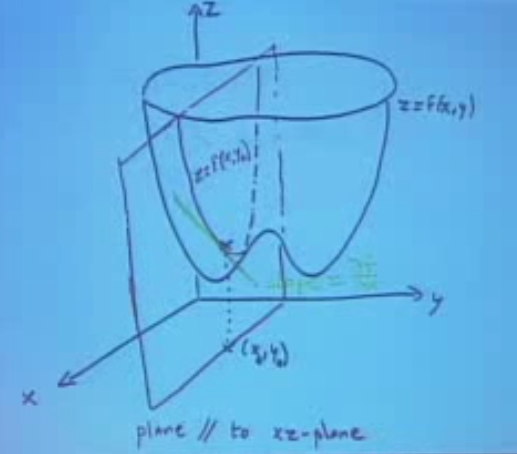
\includegraphics[height=4cm]{9_1.png}

Hatirlarsak $\frac{\partial f}{\partial x}$ kismi turevi $x$'in degistigi
ama $y$'nin sabit tutuldugu bir durumu tarif ediyordu. Yukaridaki grafige
gore bu bir anlamda iki cukurlu kap gibi duran $z$ fonksiyonun bir kesitine
bakmak gibi (unutmayalim, fonksiyon sadece kabin disinda tanimli, ici
bos). Bu kesit $f$'in bir yansimasini olusturuyor, o yansima ustteki
grafikte bir parabol seklinde. Bu parabolda $x$ degistikce o noktanin
parabol uzerindeki cizgizel tegeti de degisiyor (grafikteki yesil cizgi) ki
bu cizgisel egim $\frac{\partial f}{\partial x}$'e esit. 

Eger ayni seyi $x$'in sabit $y$'nin sabit oldugu durum icin yapsaydim,
benzer bir kesit elde edecektim. 

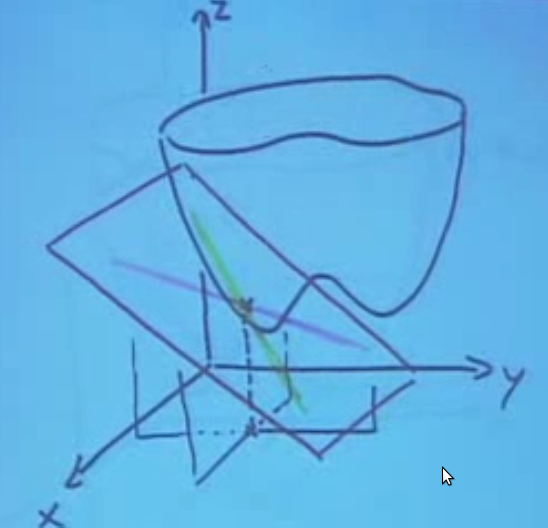
\includegraphics[height=4cm]{9_2.png}

Bu iki kesit uzerinden elde edilen ikinci teget cizgi birinci ile beraber
kullanilinca bir duzlemi tanimlamak icin kullanilabilir (iki cizgi paralel
bir duzlem tanimlamak icin yeterlidir), ki teget duzlem yaklasiksallamasi
icin kullanilacak duzlem budur. Bunu nasil yapacagimizi gosterelim.

$f_x$ ve $f_y$ iki teget cizgiyi tanimlamak icin kullaniliyorsa, bu
formulleri bir araya koyarak duzlemi temsil edebilirim. Eger

\[ \frac{\partial f}{\partial x}(x_0,y_0) = a \]

ise bu demektir ki birinci teget cizgi (yesil cizgi) $L_1$ soyledir:

\[ 
L_1 = 
\left\{ \begin{array}{l}
z = z_0 + a(x - x_0) \\
y = y_0
\end{array} \right.
 \]

Bu cizgi icin $y$'yi sabit tutuyorum, $z$'deki degisimi $z_0$ ustune egim
$a$'nin katlari kadar ($x$'in degisimi oraninda carparak) ekleyerek
hesapliyorum. 





\end{document}
